\documentclass[10pt]{article}
\usepackage[polish]{babel}
\usepackage[utf8]{inputenc}
\usepackage[T1]{fontenc}
\usepackage{graphicx}
\usepackage[export]{adjustbox}
\graphicspath{ {./images/} }
\usepackage{amsmath}
\usepackage{amsfonts}
\usepackage{amssymb}
\usepackage[version=4]{mhchem}
\usepackage{stmaryrd}

\title{LIGA MATEMATYCZNA \\
 im. Zdzisława Matuskiego \\
 GRUDZIEŃ 2013 \\
 SZKOŁA PODSTAWOWA }

\author{}
\date{}


\begin{document}
\maketitle
\section*{ZADANIE 1.}
Kwadrat o boku długości 10 cm podzielono na mniejszy kwadrat i cztery jednakowe prostokąty. Każda z pięciu części ma taki sam obwód. Oblicz pole małego kwadratu.\\
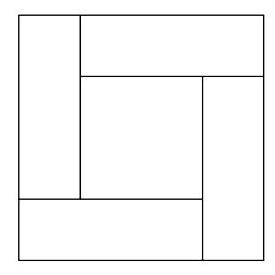
\includegraphics[max width=\textwidth, center]{2024_11_21_51f6fb0dd520436b83ddg-1}

\section*{ZADANIE 2.}
Liczbę naturalną nazywamy dobrą, jeżeli można ją zapisać przy pomocy różnych cyfr, których iloczyn jest równy 360. Podaj co najmniej dwie takie liczby naturalne. Wyznacz największą dobrą liczbę naturalną.

\section*{ZADANIE 3.}
W pięciu rzutach kostką do gry otrzymano 27 punktów. Ile razy maksymalnie mogło wypaść 6 oczek? Ile razy mogło wypaść 5 oczek?

\section*{ZADANIE 4.}
Do sklepu dostarczono gwoździe w sześciu skrzynkach. Gwoździe ważyły \(2 \mathrm{~kg}, 3 \mathrm{~kg}, 5 \mathrm{~kg}, 8 \mathrm{~kg}\), 9 kg i 10 kg . Którą skrzynkę sprzedawca powinien sprzedać panu Nowakowi, aby pozostałe 5 skrzynek można było rozdzielić między dwóch klientów tak, aby gwoździe w zakupionych przez nich skrzynkach ważyły tyle samo?

\section*{ZADANIE 5.}
Joanna, Paweł, Michał, Piotr i Jarek mieszkają w jednym bloku. Każdy z nich prowadzi inny samochód: peugeot, renault (samochody francuskie), fiat (samochód włoski), ligier (francuski samochód wyścigowy) i ferrari (włoski samochód wyścigowy). Ustal jaki samochód posiada każdy z nich, jeżeli:

\begin{itemize}
  \item Paweł i Michał mają samochody francuskie;
  \item Joanna i Jarek lubią bezpieczną jazdę i nie mają samochodów wyścigowych;
  \item Michał, Joanna i Jarek wsiadają często do renaulta, ale go nie prowadzą;
  \item Joanna, Paweł i właściciel peugeota są przyjaciółmi.
\end{itemize}

\end{document}